\documentclass[11pt,a4paper,oneside]{book}
\usepackage[utf8]{inputenc}
\usepackage[T1]{fontenc}
\usepackage{lmodern}
\usepackage[margin=2.5cm]{geometry}
\usepackage{microtype}
\usepackage{amsmath,amssymb}
\usepackage{booktabs,array}
\usepackage{xcolor}
\usepackage{enumitem}
\usepackage{listings}
\usepackage{tikz}
\usetikzlibrary{arrows.meta,positioning,calc,fit,backgrounds}
\usepackage[most]{tcolorbox}
\usepackage{caption}
\usepackage[colorlinks=true,linkcolor=blue!50!black,urlcolor=blue!50!black,citecolor=blue!50!black]{hyperref}

\setlength{\parskip}{0.5em}
\setlength{\parindent}{0pt}
\renewcommand{\arraystretch}{1.15}
\setcounter{tocdepth}{2}
\emergencystretch=2em

% ---------- macros ----------
\newcommand{\code}[1]{\texttt{\detokenize{#1}}}
\newcommand{\bits}[1]{\texttt{#1}}
\newcommand{\hex}[1]{\texttt{0x#1}}
\newcommand{\LZMA}{\textsc{lzma}}

% ---------- boxes ----------
\newtcolorbox{keyidea}[1][Key idea]{enhanced,breakable,colback=blue!4,colframe=blue!55!black,
  fonttitle=\bfseries,title={#1},boxrule=0.6pt,arc=2pt}
\newtcolorbox{workedex}[1]{enhanced,breakable,colback=green!4!white,colframe=green!40!black,
  fonttitle=\bfseries,title={Worked example: #1},boxrule=0.6pt,arc=2pt}
\newtcolorbox{pitfall}[1][Watch out]{enhanced,breakable,colback=orange!6,colframe=orange!70!black,
  fonttitle=\bfseries,title={#1},boxrule=0.6pt,arc=2pt}

% ---------- listings ----------
\lstdefinestyle{code}{basicstyle=\ttfamily\footnotesize,keywordstyle=\color{blue!60!black}\bfseries,
  commentstyle=\color{green!40!black}\itshape,stringstyle=\color{red!50!black},
  numbers=left,numberstyle=\tiny\color{gray},numbersep=6pt,frame=single,rulecolor=\color{black!30},
  breaklines=true,columns=fullflexible,keepspaces=true,showstringspaces=false,
  xleftmargin=1.6em,framexleftmargin=1.6em,aboveskip=0.8em,belowskip=0.5em}
\lstdefinelanguage{pseudo}{morekeywords={if,else,while,for,return,do,then,end,function,loop},
  sensitive=true,morecomment=[l]{//}}
\lstset{style=code}

\captionsetup{font=small,labelfont=bf}

\begin{document}

% ---------- title ----------
\begin{titlepage}
\centering
\vspace*{2.5cm}
{\Huge\bfseries LZMA Compression\\[0.3em] Explained in Detail\par}
\vspace{0.8cm}
{\Large From information theory and the range coder\\ to every bit of the packet format\par}
\vspace{1.6cm}
{\large A self-contained tutorial with worked examples,\\ verified against a reference implementation\par}
\vfill
\begin{tcolorbox}[colback=black!3,colframe=black!30,width=0.85\textwidth,left=6pt,right=6pt]
\small\raggedright
\textbf{About the examples.} Every numeric example in this document (range-coder arithmetic, probability
tables, the token trace for the 15-byte sample string, the benchmark table) was computed by running code,
and the C decoder in Appendix~A was tested against files produced by the real \texttt{xz} tool (liblzma), including text,
executable code, random data, long runs, an empty file, and several \code{lc}/\code{lp}/\code{pb} settings, under AddressSanitizer
and UBSan.
\end{tcolorbox}
\vspace{1cm}
\end{titlepage}

\frontmatter
\tableofcontents

\chapter*{How to read this document}
\addcontentsline{toc}{chapter}{How to read this document}

LZMA is the algorithm behind the \texttt{.7z} and \texttt{.xz} formats. It routinely produces files that are 20--40\%
smaller than those produced by Deflate (\texttt{gzip}, \texttt{zip}, \texttt{zlib}) and often smaller than \texttt{bzip2}.
The reason is not one clever trick but a sequence of well-chosen engineering decisions, each of which saves a
little, and which compound. This document walks through all of them.

The document is organised in three layers:

\begin{description}[leftmargin=2em,style=nextline]
\item[Foundations (Chapters 1--4)] Entropy, dictionary (LZ77) compression, and the \emph{range coder}, which is the
  engine that makes LZMA special. If you already know these, skim Chapter~4 for the exact integer arithmetic.
\item[The LZMA format (Chapters 5--10)] The packet types, the state machine, literal coding, length and distance
  coding, repeated matches, a complete end-to-end trace of a real compressed stream, and the container formats.
\item[The encoder and the big picture (Chapters 11--12)] How an encoder chooses packets (match finders, optimal
  parsing), and a quantitative account of why LZMA beats the alternatives and where it loses.
\end{description}

Chapter~13 contains exercises (with solutions), and Appendix~A contains a complete, tested LZMA decoder in about 200
lines of C. Reading that code after Chapters 4--8 is the best way to check that you really understood
everything: the decoder is the specification.

\paragraph{Conventions.}
Bits are written \bits{like this}. Hexadecimal numbers carry a \texttt{0x} prefix. ``Byte'' means 8 bits.
$\log_2$ is the base-2 logarithm. Positions in the data are counted from 0.
Probabilities inside LZMA are integers in $[0,2048)$; when we say ``probability $p$'' for such a number we mean
$p/2048$.

\mainmatter

% =====================================================================
\chapter{Introduction}
% =====================================================================

\section{What is LZMA?}

\LZMA{} stands for \emph{Lempel--Ziv--Markov chain algorithm}. It was designed by Igor Pavlov and first appeared in
the 7-Zip archiver around 2001. Its reference implementation, the LZMA SDK, is in the public domain. Today it is found in
the \texttt{.7z} archive format, in the \texttt{.xz} and \texttt{.lzma} file formats, and in many software distribution
and kernel-image formats, where one compresses once and decompresses many times.

The name describes two ingredients:

\begin{itemize}
\item \textbf{Lempel--Ziv}: a \emph{dictionary} method. The compressor replaces repeated byte strings by references
  \emph{(distance, length)} back into data it has already emitted.
\item \textbf{Markov chain}: the compressed symbols are coded using \emph{context-dependent probabilities}, where the
  context includes a small state machine that remembers the last few kinds of packets. This is what lets the
  encoder predict whether the next thing is likely to be a literal byte or a match.
\end{itemize}

\begin{keyidea}[The one-paragraph summary]
LZMA first turns the input into a stream of \emph{packets}: \textbf{literals} (a raw byte), \textbf{matches}
(copy $L$ bytes from distance $D$ back), and \textbf{repeated matches} (reuse one of the four most recent
distances). It then encodes every single decision (``is this a match?'', ``which length?'', each bit of each byte,
\dots) as a \emph{binary decision with an adaptive probability}, using a \textbf{range coder} that spends
fractions of a bit per decision when the decision is predictable. The context used to look up each probability
is carefully chosen so predictions are sharp.
\end{keyidea}

\section{The two-layer architecture}

Figure~\ref{fig:pipeline} shows the pipeline. Everything in LZMA belongs to one of two layers, and keeping them
mentally separate is the key to understanding it.

\begin{figure}[ht]
\centering
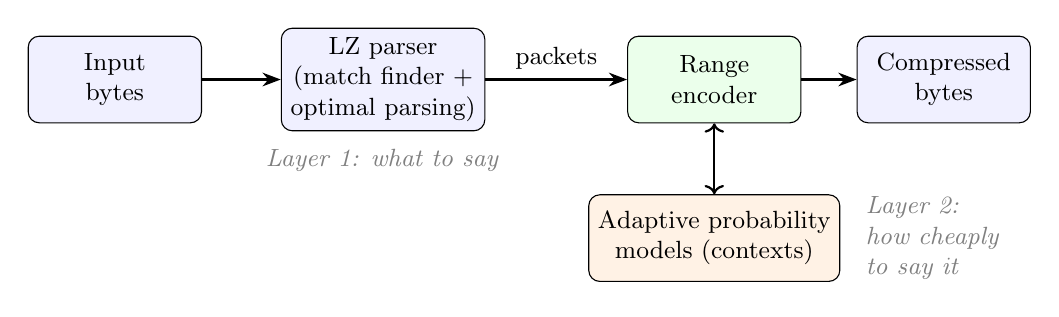
\begin{tikzpicture}[font=\small,
  box/.style={draw,rounded corners,align=center,minimum height=1.1cm,minimum width=2.2cm,fill=blue!6},
  arr/.style={-{Stealth},thick}]
\node[box] (in) {Input\\bytes};
\node[box,right=1.0cm of in] (lz) {LZ parser\\(match finder +\\ optimal parsing)};
\node[box,right=1.8cm of lz,fill=green!8] (rc) {Range\\encoder};
\node[box,right=0.7cm of rc] (out) {Compressed\\bytes};
\node[box,below=0.9cm of rc,fill=orange!10] (mod) {Adaptive probability\\models (contexts)};
\draw[arr] (in)--(lz);
\draw[arr] (lz)--node[above]{packets}(rc);
\draw[arr] (rc)--(out);
\draw[arr,<->] (rc)--(mod);
\node[below=0.1cm of lz,align=center,gray] (l1) {\textit{Layer 1: what to say}};
\node[right=0.3cm of mod,align=left,gray,xshift=-0.1cm] {\textit{Layer 2:}\\\textit{how cheaply}\\\textit{to say it}};
\end{tikzpicture}
\caption{The LZMA pipeline. Layer~1 decides \emph{what} to encode (a sequence of literals and matches).
Layer~2 decides \emph{how many bits} each decision costs, by modelling probabilities adaptively.}
\label{fig:pipeline}
\end{figure}

\textbf{Layer 1 (parsing)} is a search problem: find a good way to describe the data as literals and matches.
The format does not dictate \emph{how} the encoder does this. Any valid packet sequence decodes correctly, so encoders
are free to trade speed for quality. That freedom is why \texttt{xz -0} and \texttt{xz -9} produce
streams that every decoder can read.

\textbf{Layer 2 (entropy coding)} is a modelling problem, and it is rigidly specified by the format, because the
decoder must reproduce exactly the same probabilities as the encoder.

\section{What makes it ``beat'' other algorithms?}

A preview of the answer (made quantitative in Chapter~12):

\begin{enumerate}
\item A \textbf{huge dictionary}: Deflate looks back at most 32\,KiB; LZMA can look back megabytes to gigabytes.
\item A \textbf{range coder with adaptive binary probabilities}: no whole-bit rounding (Huffman needs at least 1 bit per
  symbol) and no side information (Huffman trees must be transmitted; LZMA's models are learned on the fly by both sides).
\item \textbf{Rich contexts}: a literal is coded knowing the previous byte; a flag is coded knowing the recent history of
  packet types and the position modulo a small power of two.
\item \textbf{Matched literals}: right after a match, the byte that \emph{would have} continued the match is used as extra
  context for the next literal.
\item \textbf{Repeated-distance packets}: the last four distances are cheap to reuse, which fits structured data
  (tables, code, records).
\item \textbf{Optimal parsing}: the encoder runs a dynamic-programming shortest-path search over the cost of
  alternative packet sequences, rather than greedily taking the longest match.
\end{enumerate}

The price is speed: compression is slow and decompression, while fast enough for most uses, is inherently sequential
and slower than Deflate or Zstandard.

% =====================================================================
\chapter{Information Theory in One Chapter}
% =====================================================================

You do not need much theory to understand LZMA, but a few ideas appear everywhere in the rest of this document.

\section{Information and entropy}

If an event has probability $p$, observing it conveys $-\log_2 p$ bits of \emph{information} (surprise). Rare events are
surprising and therefore expensive to communicate; near-certain events cost almost nothing.

\begin{center}
\begin{tabular}{rr}
\toprule
$p$ & cost $-\log_2 p$ (bits)\\
\midrule
0.5 & 1.000\\
0.9 & 0.152\\
0.985 & 0.022\\
0.1 & 3.322\\
0.01 & 6.644\\
\bottomrule
\end{tabular}
\end{center}

The \emph{entropy} of a source is the expected cost per symbol, $H=-\sum_i p_i\log_2 p_i$. Shannon's source coding theorem
says no lossless compressor can beat $H$ bits per symbol on average \emph{for a source with those probabilities}, and that
one can get arbitrarily close.

\begin{workedex}{a biased coin}
A coin shows heads with probability $0.1$. Then
\[
H = -0.9\log_2 0.9 - 0.1\log_2 0.1 \approx 0.9\cdot 0.152 + 0.1\cdot 3.322 = 0.469\ \text{bits per flip.}
\]
A naive encoding uses 1 bit per flip; an ideal coder needs only 0.469 bits per flip, a saving of 53\%.
\end{workedex}

\section{Compression is prediction}

An ideal coder spends $-\log_2 p$ bits for a symbol the model predicted with probability $p$. So the quality of
compression is exactly the quality of the \emph{predictions}. A compressor therefore has two independent jobs:

\begin{description}[leftmargin=2em]
\item[Modelling] assign a probability to every possible next event (using whatever the encoder and decoder both know).
\item[Coding] turn probabilities into bits with as little waste as possible.
\end{description}

Huffman coding is a coding method with a significant limitation: each symbol gets a whole number of bits.
If a binary decision has $P(\text{yes})=0.99$, the entropy is $H=0.081$ bits, but Huffman still spends a full bit per decision, a
\emph{twelve-fold} overhead. LZMA codes a large number of very skewed binary decisions (``is the next packet a literal?''
is true or false with high confidence in many contexts), so a coder that can spend 0.02 bits on a predictable decision
is decisive. That coder is the \textbf{range coder} of Chapter~4.

\begin{keyidea}
Huffman coding is wasteful for highly predictable binary decisions, because it cannot spend less than one bit per symbol.
Arithmetic/range coding has no such floor, and LZMA is designed to exploit this.
\end{keyidea}

% =====================================================================
\chapter{Dictionary Compression (LZ77)}
% =====================================================================

\section{The basic idea}

Real data repeats itself: words in text, identifiers in source code, instruction sequences in executables.
LZ77 (Ziv and Lempel, 1977) exploits this by keeping a \emph{window} of recently processed data (the
\emph{dictionary}) and replacing a repeated string by a pair $(D, L)$ meaning ``go back $D$ bytes and copy $L$ bytes''.

\begin{workedex}{LZ77 on \texttt{abracadabra}}
Positions: \texttt{a b r a c a d a b r a} are positions $0,\dots,10$.
Scanning left to right, the encoder emits literals for \texttt{a b r a c a d}. (At position~3, the byte
\texttt{a} matches position~0 but a length-1 match is not worth a reference.) At position~7 the string
\texttt{abra} also occurs at position~0, i.e.\ $D=7$ bytes back, with $L=4$:
\[
\underbrace{\texttt{a}\ \texttt{b}\ \texttt{r}\ \texttt{a}\ \texttt{c}\ \texttt{a}\ \texttt{d}}_{\text{7 literals}}\
\underbrace{(D{=}7,L{=}4)}_{\text{match}}
\]
Eleven bytes have become 7 literals plus one match. The decoder rebuilds the data by copying 4 bytes starting 7 bytes behind its write position.
\end{workedex}

\section{Overlapping matches and run-length behaviour}

A match is allowed to have $L>D$. The decoder copies \emph{byte by byte}, so bytes that were just written can be
copied again:

\begin{lstlisting}[language=pseudo]
function copy_match(out, D, L):
    for i in 0 .. L-1:
        out.append( out[ len(out) - D ] )     // reads bytes written a moment ago
\end{lstlisting}

For example, \texttt{aaaaaaaa} (8 bytes) is the literal \texttt{a} followed by the match $(D{=}1,L{=}7)$. A distance-1 match
therefore behaves as run-length encoding, and a distance-$k$ match repeats a $k$-byte pattern. No separate RLE mechanism is
needed.

\section{Parameters of the LZMA dictionary}

\begin{center}
\begin{tabular}{lp{2.4cm}p{8cm}}
\toprule
 & Deflate & LZMA\\
\midrule
Window (max distance) & 32 KiB & up to 4 GiB in the format (typically 1--64\,MiB in practice)\\
Minimum match length & 3 & 2\\
Maximum match length & 258 & 273\\
\bottomrule
\end{tabular}
\end{center}

The size of the window matters a great deal for large files with long-range redundancy (for example, similar source files or
sections of a binary far apart). A match finder for such a window needs good data structures (Chapter~11).

\section{Parsing: which matches should be used?}

At each position many candidate matches exist (different distances and lengths). The \emph{parsing strategy} chooses among them:

\begin{description}[leftmargin=2em]
\item[Greedy] always take the longest match available. Fast, but often suboptimal.
\item[Lazy] look one position ahead and delay if a longer match starts at the next byte. (Used by gzip.)
\item[Optimal] consider the \emph{cost in bits} of alternatives over a window of positions and choose the cheapest path.
  This is what LZMA's best compression modes do (Chapter~11).
\end{description}

\section{Why LZ77 alone is not enough}

Plain LZ77 outputs a stream of literals and $(D,L)$ pairs. Written naively (say, 1 flag bit, 8 bits per literal,
and 16+8 bits per match) it compresses only modestly. All the sophistication of modern LZ-based compressors lies in how the
packets are \emph{coded}. Deflate applies Huffman coding to the literal/length symbols and distance symbols, with trees
transmitted per block. LZMA instead uses a context-modelled adaptive range coder and a richer set of packet types. The next
chapter builds that coder.

% =====================================================================
\chapter{The Range Coder}
% =====================================================================

This is the most important chapter. Once you understand it, the LZMA format is just a long list of
\emph{which probability to use for which decision}.

\section{Arithmetic coding in one picture}

An arithmetic coder represents an entire message as a single number inside a nested sequence of shrinking intervals.
Start with the interval $[0,1)$. For each binary decision, split the current interval in proportion to the probabilities of
the two outcomes and keep the part matching the actual outcome. The final interval is narrow; any number inside it identifies the message.

\begin{workedex}{decimal toy coder}
Let $P(\text{bit}=0)=0.8$. Encode the bits $0,0,1$.
\begin{center}
\begin{tabular}{llll}
\toprule
step & bit & interval before & interval after\\
\midrule
1 & 0 & $[0,\,1)$ & $[0,\,0.8)$\\
2 & 0 & $[0,\,0.8)$ & $[0,\,0.64)$\\
3 & 1 & $[0,\,0.64)$ & $[0.512,\,0.64)$\\
\bottomrule
\end{tabular}
\end{center}
The final width is $0.8\cdot0.8\cdot0.2=0.128$, so the message costs $-\log_2 0.128=2.97$ bits. The binary fraction
$0.1001_2=0.5625$ lies inside $[0.512,0.64)$ and needs only 4 bits to write down, so a number of about
$\lceil\log_2(1/0.128)\rceil+1=4$ bits identifies the message. The cost is the information content, up to a small constant, with no
per-symbol rounding.
\end{workedex}

A \textbf{range coder} is an arithmetic coder implemented with integer arithmetic, working on bytes: it keeps a
\emph{low} end and a \emph{range} (width) in 32-bit/64-bit integers and emits bytes as soon as they are certain. LZMA uses a
\emph{binary} range coder: every decision is a single yes/no with an adaptive probability.

\section{Adaptive probabilities}

LZMA stores each probability as an 11-bit integer \code{prob} in $[0,2048)$: the probability that the next bit is \bits{0} is
$\code{prob}/2048$. Each probability starts at $1024$ (that is, $1/2$), and after every coded bit it moves towards the observed outcome:
\begin{align*}
\text{bit}=0:&\quad \code{prob} \leftarrow \code{prob} + \big(2048-\code{prob}\big)\gg 5,\\
\text{bit}=1:&\quad \code{prob} \leftarrow \code{prob} - \big(\code{prob}\gg 5\big).
\end{align*}
This is an exponentially weighted moving average with factor $31/32$: the model effectively remembers roughly the last
32 occurrences in that context.

\begin{workedex}{how fast does a probability learn?}
Starting from $\code{prob}=1024$ and seeing only zeros, $\code{prob}_n \approx 2048-1024\,(31/32)^n$.
The table below was computed by actually iterating the integer update rule.
\begin{center}
\begin{tabular}{rrrr}
\toprule
zeros seen & \code{prob} & $P(0)$ & cost of next \bits{0} (bits)\\
\midrule
0 & 1024 & 0.500 & 1.000\\
1 & 1056 & 0.516 & 0.956\\
2 & 1087 & 0.531 & 0.914\\
5 & 1174 & 0.573 & 0.803\\
10 & 1300 & 0.635 & 0.656\\
20 & 1499 & 0.732 & 0.450\\
50 & 1828 & 0.893 & 0.164\\
100 & 1990 & 0.972 & 0.041\\
$\ge 200$ & 2017 & 0.985 & 0.022\\
\bottomrule
\end{tabular}
\end{center}
\end{workedex}

\begin{keyidea}[A built-in floor]
Because of the integer shifts, \code{prob} can never exceed $2048-31=2017$ (once $2048-\code{prob}<32$ the increment
$\lfloor(2048-\code{prob})/32\rfloor$ is $0$), nor drop below $31$. So even a perfectly predictable bit costs at least
$-\log_2(2017/2048)\approx 0.022$ bits. This is not a bug: a probability that could reach 1 would make the first surprise
catastrophically expensive.
\end{keyidea}

\section{The encoder}

State: \code{low} (a 64-bit integer, only 33 bits meaningful), \code{range} (32-bit), plus a \code{cache} byte and a counter
\code{cacheSize} used for carry propagation. Initially \code{low = 0}, \code{range = 0xFFFFFFFF},
\code{cache = 0}, \code{cacheSize = 1}.

\begin{lstlisting}[language=pseudo,caption={Encoding one bit with an adaptive probability.}]
function encode_bit(prob, bit):
    bound = (range >> 11) * prob          // size of the "bit = 0" sub-interval
    if bit == 0:
        range = bound
        prob  = prob + ((2048 - prob) >> 5)
    else:
        low   = low + bound               // skip past the "0" part
        range = range - bound
        prob  = prob - (prob >> 5)
    while range < 2^24:                   // normalize: keep range large
        range = range << 8
        shift_low()
\end{lstlisting}

The probability occupies the \emph{lower} part of the interval (the \bits{0} outcome) and the \bits{1} outcome the
remainder. Note that $\code{range}\gg 11$ first discards 11 low bits so the product with an 11-bit \code{prob} cannot overflow
32 bits.

\begin{lstlisting}[language=pseudo,caption={Emitting bytes and propagating carries.}]
function shift_low():
    if low < 0xFF000000 or low >= 2^32:          // top byte is now certain (or a carry occurred)
        carry = low >> 32                         // 0 or 1
        temp  = cache
        do:
            output_byte( (temp + carry) & 0xFF )
            temp = 0xFF
        while --cacheSize != 0
        cache = (low >> 24) & 0xFF
    cacheSize += 1
    low = (low & 0x00FFFFFF) << 8
\end{lstlisting}

Why the cache? Adding \code{bound} to \code{low} can overflow into bit 32 (a \emph{carry}) that must be added to a byte that
may already have been ``almost'' emitted. The coder therefore holds back the most recent byte (\code{cache}) together with a
run of \hex{FF} bytes (\code{cacheSize}$-1$ of them), since only those can change if a carry arrives. This also explains a
curious fact: \textbf{the first byte of every LZMA range-coded stream is \hex{00}}, because the very first byte shifted out is
the initial \code{cache}.

At the end the encoder calls \code{shift_low()} five times to flush everything.

\section{The decoder}

The decoder mirrors the encoder but keeps \code{code}, the difference between the received number and \code{low}. Initially it
reads 5 bytes (the first must be \hex{00}), setting \code{range = 0xFFFFFFFF} and \code{code} to the next 4 bytes read big-endian.

\begin{lstlisting}[language=pseudo,caption={Decoding one bit.}]
function decode_bit(prob):
    bound = (range >> 11) * prob
    if code < bound:                      // falls in the "0" part
        range = bound
        prob  = prob + ((2048 - prob) >> 5)
        bit = 0
    else:
        range = range - bound
        code  = code - bound
        prob  = prob - (prob >> 5)
        bit = 1
    if range < 2^24:                      // normalize
        range = range << 8
        code  = (code << 8) | next_input_byte()
    return bit
\end{lstlisting}

The decoder only needs to \emph{compare} \code{code} with \code{bound}. It performs exactly the same
\code{prob} and \code{range} updates as the encoder, which is why the two stay synchronised without ever communicating
probabilities.

\section{Numeric trace}

Let us encode the three bits $0,0,1$ starting from a fresh probability $\code{prob}=1024$ and
$\code{range}=\hex{FFFFFFFF}=4\,294\,967\,295$. (The following values were produced by running the algorithm.)

\begin{center}
\small
\begin{tabular}{rrrrrr}
\toprule
bit & \code{prob} before & \code{bound} & \code{range} after & \code{low} after & \code{prob} after\\
\midrule
0 & 1024 & 2\,147\,482\,624 & 2\,147\,482\,624 & 0 & 1056\\
0 & 1056 & 1\,107\,295\,200 & 1\,107\,295\,200 & 0 & 1087\\
1 & 1087 &   587\,709\,377 &   519\,585\,823 & 587\,709\,377 & 1054\\
\bottomrule
\end{tabular}
\end{center}

Step~1: $\code{range}\gg11=2\,097\,151$ and $2\,097\,151\times1024=2\,147\,482\,624$. Step~2 uses the new probability $1056$:
$(2\,147\,482\,624\gg 11)\times1056=1\,048\,575\times1056=1\,107\,295\,200$. Step~3: the bit is \bits{1}, so \code{low} jumps up by \code{bound} and the new
range is the remainder, $1\,107\,295\,200-587\,709\,377=519\,585\,823$. No normalisation was needed since the range is still above $2^{24}=16\,777\,216$.

\begin{figure}[ht]
\centering
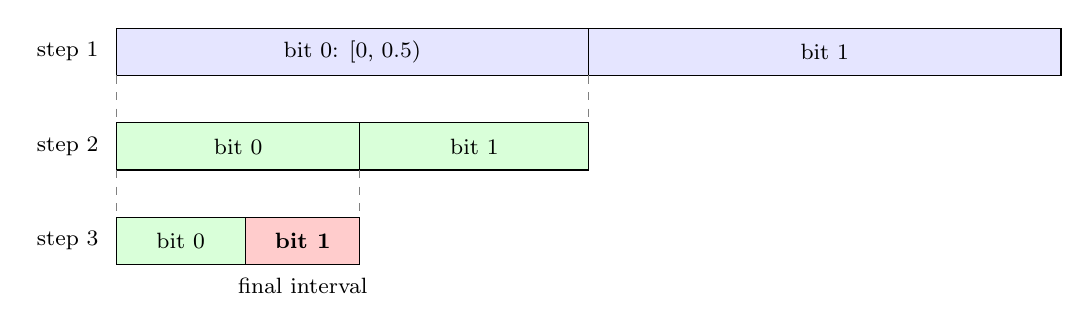
\begin{tikzpicture}[x=1cm,y=1cm,font=\footnotesize]
% full-scale: 12 cm = 2^32
\def\W{12}
\fill[blue!10] (0,2.4) rectangle (\W,3.0);
\draw (0,2.4) rectangle (\W,3.0);
\draw (6.0,2.4)--(6.0,3.0);
\node at (3,2.7) {bit 0: $[0,\,0.5)$};
\node at (9,2.7) {bit 1};
\node[left] at (-0.1,2.7) {step 1};

\fill[green!15] (0,1.2) rectangle (6.0,1.8);
\draw (0,1.2) rectangle (6.0,1.8);
\draw (3.094,1.2)--(3.094,1.8);
\node at (1.55,1.5) {bit 0};
\node at (4.55,1.5) {bit 1};
\node[left] at (-0.1,1.5) {step 2};

\fill[green!15] (0,0) rectangle (3.094,0.6);
\draw (0,0) rectangle (3.094,0.6);
\draw (1.642,0)--(1.642,0.6);
\fill[red!20] (1.642,0) rectangle (3.094,0.6);
\draw (1.642,0) rectangle (3.094,0.6);
\node at (0.82,0.3) {bit 0};
\node at (2.37,0.3) {\bfseries bit 1};
\node[left] at (-0.1,0.3) {step 3};

\draw[dashed,gray] (0,2.4)--(0,1.8);
\draw[dashed,gray] (6.0,2.4)--(6.0,1.8);
\draw[dashed,gray] (0,1.2)--(0,0.6);
\draw[dashed,gray] (3.094,1.2)--(3.094,0.6);
\node[below] at (2.37,-0.05) {final interval};
\end{tikzpicture}
\caption{Interval narrowing for the bits $0,0,1$ (drawn to scale: the full bar is $2^{32}$ wide). At each step the current
interval is split at \code{bound}; the part matching the coded bit becomes the next interval. The final interval is about
12.1\% of the original, i.e.\ $3.05$ bits of information, which is exactly the sum of the three modelled costs
$1.000+0.956+1.092$ (the third bit is a ``surprise'' because the model had learned to expect a \bits{0}).}
\end{figure}

\section{Normalisation and precision}

The coder maintains $\code{range}\ge2^{24}$ after every step. Since $\code{prob}\in[31,2017]$ and
$\code{range}\gg 11\ge2^{13}$, both sub-intervals $\code{bound}$ and $\code{range}-\code{bound}$ are non-empty. The use of $\code{range}\gg11$
truncates a little, which costs a tiny amount of efficiency (relative error below $2^{-13}$ per decision); in return
everything fits in 32-bit multiplication.

When the range falls below $2^{24}$ the coder shifts a byte out (encoder) or in (decoder). On average the stream therefore
grows exactly as fast as the information content requires, in units of whole bytes but with \emph{fractional bits} accumulated
across decisions in \code{range}.

\section{Coding multi-bit values}

The binary coder codes one bit at a time. For larger values LZMA uses three constructions.

\subsection{Bit trees}
To code an $m$-bit value from most significant bit to least, use $2^m$ probabilities arranged as a binary tree. The
index starts at \code{m = 1}; after coding a bit $b$, set $\code{m} \leftarrow 2\code{m}+b$. The probability used for each bit is
\code{probs[m]} \emph{before} the update. Because the index records all the earlier bits, each bit is predicted given the bits above it,
so the tree learns an arbitrary distribution over the $2^m$ values.

\begin{workedex}{bit tree, 3 bits, value 5}
$5=\bits{101}$. Start $\code{m}=1$.
\begin{center}
\begin{tabular}{ccc}
\toprule
bit & probability used & new \code{m}\\
\midrule
\bits{1} & \code{probs[1]} & $3$\\
\bits{0} & \code{probs[3]} & $6$\\
\bits{1} & \code{probs[6]} & $13$\\
\bottomrule
\end{tabular}
\end{center}
Finally the value is $\code{m}-2^3=13-8=5$. Different values touch different probabilities, so common values become cheap.
\end{workedex}

\subsection{Reverse bit trees}
Identical, except that the bits are coded from the \emph{least} significant bit to the most significant. Coding value $6=\bits{110}$:
bits $0,1,1$ use \code{probs[1]}, \code{probs[2]}, \code{probs[5]} ($\code{m}:1\to2\to5\to11$), and the value is rebuilt as $\sum b_i 2^i$.
LZMA uses these for the low bits of distances, where the low bits are better predicted from each other than from the high bits.

\subsection{Direct bits}
Some bits are essentially random (the middle bits of large distances). These are coded with a fixed probability of $1/2$, with no model and no adaptation:
\begin{lstlisting}[language=pseudo]
function encode_direct_bits(value, n):
    for i from n-1 down to 0:
        range = range >> 1
        if (value >> i) & 1: low = low + range
        normalize()
\end{lstlisting}
Each such bit costs exactly one bit.

\begin{pitfall}[Two meanings of ``bit'']
``Bit'' can mean a bit of the data being compressed or a binary decision being coded. For the range coder there is no
difference: every decision, whether a flag, a bit of a byte, or a bit of a length, is just ``code this bit using this probability slot''.
Everything LZMA does is therefore about \emph{choosing the probability slot}.
\end{pitfall}

% =====================================================================
\chapter{LZMA Packets, State and Contexts}
% =====================================================================

\section{The packet types}

An LZMA stream (after range decoding) is a sequence of packets. There are exactly seven kinds, distinguished by a short
prefix of binary decisions, \emph{each of which is coded with its own adaptive probability}:

\begin{center}
\begin{tabular}{llp{6.2cm}}
\toprule
decisions & packet & meaning\\
\midrule
\bits{0} & \textsf{LIT} & one literal byte follows\\
\bits{1 0} & \textsf{MATCH} & new match: length, then distance (stored as $D-1$)\\
\bits{1 1 0 0} & \textsf{SHORTREP} & one byte copied from distance \code{rep0}\\
\bits{1 1 0 1} & \textsf{LONGREP[0]} & match of length $\ge2$ at distance \code{rep0}\\
\bits{1 1 1 0} & \textsf{LONGREP[1]} & match at distance \code{rep1}\\
\bits{1 1 1 1 0} & \textsf{LONGREP[2]} & match at distance \code{rep2}\\
\bits{1 1 1 1 1} & \textsf{LONGREP[3]} & match at distance \code{rep3}\\
\bottomrule
\end{tabular}
\end{center}

The decisions are made, in order, with these probability arrays: \code{isMatch}, \code{isRep}, \code{isRepG0},
\code{isRep0Long}, \code{isRepG1}, \code{isRepG2}. (``G'' stands for ``greater than'': \code{isRepG0}=1 means ``not rep0''.)

\begin{lstlisting}[language=pseudo,caption={Decision tree for choosing a packet type (decoder view).}]
if decode_bit(isMatch[state][posState]) == 0:           -> LITERAL
else if decode_bit(isRep[state]) == 0:                  -> MATCH
else if decode_bit(isRepG0[state]) == 0:
    if decode_bit(isRep0Long[state][posState]) == 0:    -> SHORTREP
    else:                                               -> LONGREP[0]
else if decode_bit(isRepG1[state]) == 0:                -> LONGREP[1]
else if decode_bit(isRepG2[state]) == 0:                -> LONGREP[2]
else:                                                   -> LONGREP[3]
\end{lstlisting}

Notice the Huffman-like shape: the most common packets (literals, new matches) are reached with the fewest decisions, but the
whole tree is adaptive. If a file has many \textsf{LONGREP[1]} packets, those probabilities become sharp and they become cheap.

\section{The state variable}

The decisions above are conditioned on a \textbf{state} $\in\{0,\dots,11\}$, which summarises the last few packet types. It is a tiny
Markov chain (hence the ``M'' in LZMA). Its purpose is to allow the model to learn statements like ``after two literals, another literal is
likely'' or ``right after a match, a literal is likely, and it is likely to differ from what the match would have predicted''.

State transitions depend only on the packet just coded:
\begin{align*}
\text{after LIT:}&\quad s\mapsto \begin{cases}0 & s<4\\ s-3 & 4\le s<10\\ s-6 & s\ge10\end{cases}\\
\text{after MATCH:}&\quad s\mapsto \begin{cases}7 & s<7\\ 10 & s\ge7\end{cases}\\
\text{after LONGREP:}&\quad s\mapsto \begin{cases}8 & s<7\\ 11 & s\ge7\end{cases}\\
\text{after SHORTREP:}&\quad s\mapsto \begin{cases}9 & s<7\\ 11 & s\ge7\end{cases}
\end{align*}

\begin{center}
\small
\begin{tabular}{rlcccc}
\toprule
$s$ & recent history (oldest $\to$ newest) & LIT & MATCH & LONGREP & SHORTREP\\
\midrule
0 & LIT, LIT & 0 & 7 & 8 & 9\\
1 & MATCH, LIT, LIT & 0 & 7 & 8 & 9\\
2 & REP, LIT, LIT & 0 & 7 & 8 & 9\\
3 & SHORTREP, LIT, LIT & 0 & 7 & 8 & 9\\
4 & MATCH, LIT & 1 & 7 & 8 & 9\\
5 & REP, LIT & 2 & 7 & 8 & 9\\
6 & SHORTREP, LIT & 3 & 7 & 8 & 9\\
7 & LIT, MATCH & 4 & 10 & 11 & 11\\
8 & LIT, LONGREP & 5 & 10 & 11 & 11\\
9 & LIT, SHORTREP & 6 & 10 & 11 & 11\\
10 & non-LIT, MATCH & 4 & 10 & 11 & 11\\
11 & non-LIT, REP & 5 & 10 & 11 & 11\\
\bottomrule
\end{tabular}
\end{center}

\textbf{Rule of thumb:} states $0$--$6$ mean ``the last packet was a literal''; states $7$--$11$ mean ``the last packet was a match or rep''.
This split matters in Chapter~6 (matched literals) and in the updates above.

\section{Position state: \code{pb}}

Many files have structure at power-of-two alignments (32-bit words, 16-byte records, text lines padded to a width). LZMA conditions the
flags and lengths on $\code{posState}=\text{pos}\mathbin{\&}(2^{\code{pb}}-1)$, where pos is the number of bytes decoded so far (the position
of the \emph{start} of the packet). The default is $\code{pb}=2$ (four position classes).

\section{The three tunable parameters}

The format has three parameters, encoded in one properties byte:
\[
\code{props} = (\code{pb}\times5+\code{lp})\times9+\code{lc}.
\]
\begin{center}
\begin{tabular}{llp{10cm}}
\toprule
param & default & meaning\\
\midrule
\code{lc} & 3 & number of high bits of the \emph{previous byte} used as literal context ($0\le\code{lc}\le8$)\\
\code{lp} & 0 & number of low bits of the \emph{position} used as literal context ($0\le\code{lp}\le4$)\\
\code{pb} & 2 & number of low bits of the position used as \code{posState} ($0\le\code{pb}\le4$)\\
\bottomrule
\end{tabular}
\end{center}
The default properties byte is $(2\cdot5+0)\cdot9+3=93=\hex{5D}$, the value you will see as the first byte of nearly every \texttt{.lzma} file.
Typical tuning: keep the defaults for general data; for 32-bit aligned binary data a common suggestion is $\code{lc}=0,\ \code{lp}=2,\ \code{pb}=2$. These are only hints; the right values depend on the data and are best found by measuring.

% =====================================================================
\chapter{Literals}
% =====================================================================

\section{Plain literals}

A literal is a byte coded with an 8-level \textbf{bit tree} (Chapter~4), with a \emph{separate tree for every literal context}.
The context is
\[
\code{litState} = \big((\text{pos}\mathbin{\&}(2^{\code{lp}}-1))\ll\code{lc}\big)\ +\ (\text{prevByte}\gg(8-\code{lc})).
\]
With the defaults ($\code{lc}=3$, $\code{lp}=0$) this is simply the top 3 bits of the previous byte, giving 8 contexts. Each context has $\hex{300}=768$
probabilities (a 256-leaf tree needs 255 nodes; the rest is used by matched literals, below). In English text, the top bits of the previous byte
distinguish, for example, lowercase letters from spaces and punctuation, which helps predict the next byte's class.

\begin{keyidea}[Why only 3 high bits?]
Using the full previous byte would give 256 contexts of 768 probabilities each ($\approx$196\,608 probabilities): too many to learn from a file of ordinary size, because every context
starts at 50/50 and must be trained. Three bits is a compromise between precision and learning speed. That is why \code{lc} is a tunable parameter.
\end{keyidea}

\section{Matched literals}

Suppose the previous packet was a match (state $\ge7$) and the next byte is a literal. Intuitively: the match ended because the byte at
the copy source differs from the actual byte. But usually they are \emph{similar} (differing in just a few low bits, as with consecutive characters or numbers).
Let \code{matchByte} be the byte at distance $\code{rep0}+1$, i.e.\ what the match \emph{would} have produced next.

LZMA uses \code{matchByte} as extra context while coding the literal bit by bit from the top:

\begin{lstlisting}[language=pseudo,caption={Matched literal decoding (state $\ge$ 7).}]
sym = 1
while sym < 0x100:
    matchBit = (matchByte >> 7) & 1;  matchByte = matchByte << 1
    bit = decode_bit( probs[ ((1 + matchBit) << 8) + sym ] )
    sym = (sym << 1) | bit
    if matchBit != bit: break              // from here on, matchByte is useless
while sym < 0x100:                          // finish with the ordinary tree
    sym = (sym << 1) | decode_bit( probs[sym] )
byte = sym & 0xFF
\end{lstlisting}

The probability index has three disjoint regions: $\code{sym}$ alone (plain tree, indices $<256$), $256+\code{sym}$ (the expected bit was \bits{0}) and $512+\code{sym}$
(expected \bits{1}). So while the literal agrees with \code{matchByte}, each bit is predicted ``given that the expected bit is $m$'', which becomes a sharp
prediction (``the bit equals the match bit''). After the first disagreement the coder falls back to an ordinary tree.

\begin{workedex}{matched literals in the sample string}
In the string \texttt{abcdXabcdYabcdZ} (Chapter~9) the match \texttt{abcd} at position 5 is followed by the literal \texttt{Y}, while the byte after the
source copy is \texttt{X}. The two bytes are $\hex{59}=\bits{01011001}$ and $\hex{58}=\bits{01011000}$.
\begin{center}
\small
\begin{tabular}{rllcll}
\toprule
bit \# & \code{sym} so far & expected (matchBit) & actual & \code{probs} index & mode\\
\midrule
7 (MSB) & \bits{1} & 0 & 0 & $256+1=257$ & matched\\
6 & \bits{10} & 1 & 1 & $512+2=514$ & matched\\
5 & \bits{101} & 0 & 0 & $256+5=261$ & matched\\
4 & \bits{1010} & 1 & 1 & $512+10=522$ & matched\\
3 & \bits{10101} & 1 & 1 & $512+21=533$ & matched\\
2 & \bits{101011} & 0 & 0 & $256+43=299$ & matched\\
1 & \bits{1010110} & 0 & 0 & $256+86=342$ & matched\\
0 (LSB) & \bits{10101100} & 0 & \textbf{1} & $256+172=428$ & mismatch, done\\
\bottomrule
\end{tabular}
\end{center}
Seven bits were ``predicted'' from the match byte. In a real file, after many matches those probability slots would hold strong beliefs like ``when the
expected bit is 1 the actual bit is almost always 1'', and the cost of those seven bits becomes a few hundredths of a bit each.
\end{workedex}

\begin{workedex}{a mismatch earlier in the byte}
The final literal \texttt{Z} ($\hex{5A}=\bits{01011010}$) follows a rep match whose source continuation is \texttt{Y} ($\bits{01011001}$). The two agree for
the first 6 bits, differ at bit 1 (expected \bits{0}, actual \bits{1}), and the last bit is then coded with the plain tree at index
$\bits{10101101}=173$. (The first six rows of the table are the same as above, the seventh has index $256+86=342$ with the actual bit \bits{1}.)
\end{workedex}

\section{Why this helps}

After a match ends, the next byte is not random: it is the byte that \emph{almost} continued the match. Differences between
similar strings are often in the low bits (for instance \texttt{X} vs.\ \texttt{Y}, or a changed digit). Coding the high bits ``relative to'' the match byte
spends far fewer bits than coding the byte from scratch. This is one of the main single sources of LZMA's advantage over Deflate, which has no
such mechanism.

% =====================================================================
\chapter{Match Lengths and Distances}
% =====================================================================

\section{The length coder}

Lengths range from 2 to 273 ($=18+255$). They are split into three ranges, each with its own model; a \emph{choice}
bit and a \emph{choice2} bit select the range. Short lengths are the most common and get a cheap, \code{posState}-dependent coding.

\begin{center}
\begin{tabular}{lll}
\toprule
decisions & length range & model\\
\midrule
\code{choice}=\bits{0} & $2\ldots9$ & 3-bit tree \code{low[posState]}, value $L-2$\\
\code{choice}=\bits{1}, \code{choice2}=\bits{0} & $10\ldots17$ & 3-bit tree \code{mid[posState]}, value $L-10$\\
\code{choice}=\bits{1}, \code{choice2}=\bits{1} & $18\ldots273$ & 8-bit tree \code{high}, value $L-18$\\
\bottomrule
\end{tabular}
\end{center}

\begin{workedex}{coding lengths}
\begin{itemize}
\item $L=4$: \code{choice}=\bits{0}; \code{low} tree value $4-2=2=\bits{010}$. Cost: 4 decisions.
\item $L=12$: \code{choice}=\bits{1}, \code{choice2}=\bits{0}; \code{mid} tree value $12-10=2=\bits{010}$. Cost: 5 decisions.
\item $L=100$: \code{choice}=\bits{1}, \code{choice2}=\bits{1}; \code{high} tree value $100-18=82=\bits{01010010}$. Cost: 10 decisions.
\item $L=273$: \code{high} value $255=\bits{11111111}$ (the maximum).
\end{itemize}
\end{workedex}

There are two separate length coders: one for ordinary matches and one for repeated matches (they have different statistics).

\section{The distance coder}

The distance $D\ge1$ is stored as $d=D-1\ge0$. The key observation: distances are spread roughly logarithmically, and the exact low bits of a large distance
are mostly noise, while the magnitude (the \emph{number of bits}) is predictable. So LZMA splits $d$ into a \emph{slot} (describing the magnitude and the
second-highest bit) and \emph{extra bits}.

\paragraph{Slot.} For $d<4$, $\text{slot}=d$. For $d\ge4$, let $n=\lfloor\log_2 d\rfloor$ (position of the highest set bit) and let $b$ be the next bit below it:
\[
\text{slot}=2n+b.
\]
The slot is a 6-bit value (0--63) coded with a 6-level bit tree, using one of 4 trees selected by $\code{lenState}=\min(L-2,3)$. (Short matches have different distance
statistics than long ones: a 2-byte match is only worthwhile at small distances.)

\paragraph{Extra bits.} A slot $\ge4$ carries $n_x=(\text{slot}\gg1)-1$ extra bits, and the slot determines the base value
$\text{base}=(2\mid(\text{slot}\mathbin{\&}1))\ll n_x$. The extra bits are $d-\text{base}$ (an $n_x$-bit number). How they are coded depends on the slot:
\begin{itemize}
\item \textbf{Slots 4--13} (distances $<128$): all $n_x$ bits with a \emph{reverse bit tree} from \code{posSpecial} (adaptive).
\item \textbf{Slots 14--63}: the top $n_x-4$ bits as \emph{direct bits} (probability $1/2$, 1 bit each) and the low 4 bits with a reverse bit tree \code{align} (adaptive).
\end{itemize}

\begin{center}
\small
\begin{tabular}{rrrl}
\toprule
slot & $n_x$ extra bits & range of $d=D-1$ & coding of extra bits\\
\midrule
0--3 & 0 & $d=$ slot & none\\
4 & 1 & 4--5 & reverse tree\\
5 & 1 & 6--7 & reverse tree\\
6 & 2 & 8--11 & reverse tree\\
7 & 2 & 12--15 & reverse tree\\
8 & 3 & 16--23 & reverse tree\\
10 & 4 & 32--47 & reverse tree\\
12 & 5 & 64--95 & reverse tree\\
13 & 5 & 96--127 & reverse tree\\
14 & 6 & 128--191 & 2 direct + 4 align\\
19 & 8 & 768--1023 & 4 direct + 4 align\\
31 & 14 & 49152--65535 & 10 direct + 4 align\\
39 & 18 & 786432--1048575 & 14 direct + 4 align\\
63 & 30 & $3\cdot2^{30}$--$2^{32}-1$ & 26 direct + 4 align\\
\bottomrule
\end{tabular}
\end{center}

\begin{workedex}{distance 5 and distance 1000}
\textbf{$D=5$:} $d=4=\bits{100}$, $n=2$, next bit $b=0$, slot $=4$. $n_x=(4\gg1)-1=1$, base $=2\ll1=4$, extra $=0$. Coded: slot \bits{000100} in the slot tree for the
given \code{lenState}, then the 1-bit reverse tree with value \bits{0}.

\textbf{$D=1000$:} $d=999=\bits{1111100111}$ (10 bits). $n=9$, next bit $b=1$, slot $=2\cdot9+1=19$. $n_x=(19\gg1)-1=8$,
base $=(2\mid1)\ll8=768$, extra $=999-768=231=\bits{11100111}$. Since slot $\ge14$: the top $8-4=4$ extra bits \bits{1110} are direct bits
(4 bits cost) and the low 4 bits \bits{0111} are coded LSB-first (\bits{1,1,1,0}) in the \code{align} reverse tree. Total: 6 slot-tree decisions + 4 direct bits + 4 align decisions.
\end{workedex}

\begin{keyidea}[Why this design is smart]
The slot tree learns the \emph{distribution of distance magnitudes} (cheaply, since only 64 symbols). The align bits capture
the common pattern that distances are often multiples of 2, 4, 8 or 16 in structured data. The direct bits are the truly unpredictable
part and are sent essentially raw, at cost of exactly 1 bit each, without polluting the models.
\end{keyidea}

\section{End marker}

Distance $d=\hex{FFFFFFFF}$ (slot 63, all extra bits 1) is not a valid distance; it is used as an \emph{end-of-payload marker}. Streams of unknown
length end with it (a match packet with this distance). Streams that store their size in the header may omit it.

% =====================================================================
\chapter{Repeated Matches}
% =====================================================================

The decoder keeps the four most recently used distances \code{rep0}, \code{rep1}, \code{rep2}, \code{rep3} (initially all 0, meaning distance 1).
Data with structure repeats \emph{distances}: a table with fixed-size records, UTF-16 text, a source file where similar lines are always the same
number of bytes back, or a match interrupted by a single changed byte and then resumed at the same distance.

\begin{itemize}
\item \textbf{MATCH} (new distance): shift the history, $\code{rep3}\leftarrow\code{rep2}\leftarrow\code{rep1}\leftarrow\code{rep0}\leftarrow d$.
\item \textbf{LONGREP[$k$]}: use $\code{rep}_k$, move it to the front (the others keep relative order), and code only the \emph{length}, with the separate repeated-match length coder.
\item \textbf{SHORTREP}: copy exactly one byte from $\code{rep0}$ (no length coded). This is the cheapest nontrivial packet, useful when the byte after a match happens to equal the byte at distance $\code{rep0}$, that is, a repeat match of length 1, which a LONGREP (minimum length 2) cannot express.
\end{itemize}

\begin{workedex}{rep distance cost}
Coding a repeat of the previous match's distance takes, at 50/50 probabilities, 4 decisions for the packet type (\code{isMatch}=1, \code{isRep}=1, \code{isRepG0}=0,
\code{isRep0Long}=1) plus the length (4 decisions for $L=4$): 8 bits. A fresh match of $D=1000$ would cost 2 (type) + 4 (length) + 6 (slot) + 8 (extra) = 20 bits. After
adaptation the type decisions shrink to fractions of a bit, so a rep match can cost around 1--3 bits where a fresh match costs 15--25 bits.
\end{workedex}

This is why the encoder's optimal parser (Chapter~11) loves rep matches: a short rep match can be \emph{cheaper than a single literal}.

% =====================================================================
\chapter{A Complete Worked Example}
% =====================================================================

Let us now follow a real compression end to end. The input is the 15-byte string
\[
\texttt{abcdXabcdYabcdZ}
\]
compressed with the real liblzma (preset 6, \texttt{.lzma} format, defaults $\code{lc}=3,\ \code{lp}=0,\ \code{pb}=2$). I decoded the output with my instrumented
reference decoder to recover the exact packets the encoder chose.

\section{The packets chosen by the encoder}

\begin{center}
\small
\begin{tabular}{rrrlll}
\toprule
pos & posState & state before & packet & bytes produced & state after\\
\midrule
0 & 0 & 0 & LIT \texttt{a} & \texttt{a} & 0\\
1 & 1 & 0 & LIT \texttt{b} & \texttt{b} & 0\\
2 & 2 & 0 & LIT \texttt{c} & \texttt{c} & 0\\
3 & 3 & 0 & LIT \texttt{d} & \texttt{d} & 0\\
4 & 0 & 0 & LIT \texttt{X} & \texttt{X} & 0\\
5 & 1 & 0 & MATCH $L=4$, $D=5$ & \texttt{abcd} & 7\\
9 & 1 & 7 & LIT \texttt{Y} (matched, expected \texttt{X}) & \texttt{Y} & 4\\
10 & 2 & 4 & LONGREP[0], $L=4$ ($D=5$ again) & \texttt{abcd} & 8\\
14 & 2 & 8 & LIT \texttt{Z} (matched, expected \texttt{Y}) & \texttt{Z} & 5\\
\bottomrule
\end{tabular}
\end{center}

\section{What was coded for each packet}

\begin{enumerate}[leftmargin=2em]
\item \textbf{Pos 0--4, five literals.} For each: \code{isMatch[0][posState]}=\bits{0}, then 8 bits through the literal tree of $\code{litState}=\text{prevByte}\gg5$. For \texttt{a} the previous
  byte is taken to be 0, so $\code{litState}=0$; for the rest, the previous byte is \texttt{a},\texttt{b},\texttt{c},\texttt{d}, with $\hex{61}\gg5=\hex{62}\gg5=\hex{63}\gg5=\hex{64}\gg5=3$, so they
  all share context 3. (Letters share a context, which is exactly the point of using only high bits.)
\item \textbf{Pos 5, the match.} \code{isMatch[0][1]}=\bits{1}; \code{isRep[0]}=\bits{0} (a new distance); length: \code{choice}=\bits{0} and \code{low[1]} value $4-2=2=\bits{010}$; distance: $D=5\Rightarrow d=4$, slot 4,
  with $\code{lenState}=\min(4-2,3)=2$, slot tree \code{posSlot[2]} coding \bits{000100}, then the 1-bit reverse tree from \code{posSpecial} with value \bits{0}. State $0\to7$, $\code{rep0}=4$.
\item \textbf{Pos 9, a literal in state 7.} \code{isMatch[7][1]}=\bits{0}. State $\ge7$ so it is a \emph{matched literal}: $\code{matchByte}=\text{out}[9-(\code{rep0}+1)]=\text{out}[4]=\texttt{X}$.
  This is exactly the table of Chapter~6. State $7\to4$ (rule: $4\le s<10\Rightarrow s-3$).
\item \textbf{Pos 10, the rep match.} \code{isMatch[4][2]}=\bits{1}, \code{isRep[4]}=\bits{1}, \code{isRepG0[4]}=\bits{0}, \code{isRep0Long[4][2]}=\bits{1}; length via the \emph{repeat-length} coder: \code{choice}=\bits{0}, \code{low[2]}=\bits{010}.
  State $4\to8$. (A fresh match with $D=5$ would also have worked but is more expensive: it needs the slot and extra bits as well as the type bits.)
\item \textbf{Pos 14, last literal.} \code{isMatch[8][2]}=\bits{0}; matched literal with $\code{matchByte}=\text{out}[14-5]=\texttt{Y}$; state $8\to5$.
\item \textbf{End marker.} Because this \texttt{.lzma} stream has unknown size in its header, the encoder appends a match packet with distance \hex{FFFFFFFF}.
\end{enumerate}

\section{The actual bytes}

The compressed file is 33 bytes:
\begin{center}
\small\ttfamily
5d\ 00 00 80 00\ ff ff ff ff ff ff ff ff\ 00 30 98 88 98 3d fe f2 3b 80 dd d4 44 e0 7f ff f8 1b 20 00
\end{center}
\begin{itemize}
\item \texttt{5d}: properties byte ($\code{lc}=3,\code{lp}=0,\code{pb}=2$).
\item \texttt{00 00 80 00}: dictionary size, little-endian $=\hex{00800000}=8$\,MiB.
\item eight \texttt{ff}: uncompressed size unknown ($2^{64}-1$), so an end marker follows the data.
\item the remaining 20 bytes are the range-coded payload. The first is the mandatory \hex{00}.
\end{itemize}

\begin{pitfall}[Why did 15 bytes become 33?]
Tiny inputs cannot be compressed: the 13-byte header alone nearly doubles it, and every probability starts at $1/2$, so each early decision costs a full bit.
A rough count: five literals $\approx5\times9=45$ bits, the match $\approx13$ bits, the first matched literal $\approx9$, the rep $\approx8$, the last literal $\approx9$, and the end marker
$\approx42$ (type, length, slot and 30 distance bits). That is about 126 bits $\approx16$ bytes, and the flush of the range coder adds the rest of the 20 bytes.
Adaptive modelling only pays off once the models have been trained on a few kilobytes. The gains in Chapter~12 are measured on megabytes.
\end{pitfall}

You can now follow the example in Appendix~A: save these 33 bytes as a file and run the C decoder on it; it writes out \texttt{abcdXabcdYabcdZ}.
A good exercise is to add a \code{printf} to the decoder's main loop and watch it print exactly the packet table above.

% =====================================================================
\chapter{Container Formats}
% =====================================================================

The range-coded payload described so far is wrapped in one of several containers.

\section{The \texttt{.lzma} (LZMA-alone) format}

A 13-byte header followed by the range-coded data:
\begin{center}
\begin{tabular}{rll}
\toprule
bytes & field & notes\\
\midrule
1 & properties & $(\code{pb}\cdot5+\code{lp})\cdot9+\code{lc}$, typically \hex{5D}\\
4 & dictionary size & little-endian; typically a power of two\\
8 & uncompressed size & little-endian; all \hex{FF} means unknown (end marker required)\\
\bottomrule
\end{tabular}
\end{center}
It has no checksum and no framing, so it is mostly of historical interest; but it is exactly the format that Appendix~A decodes.

\section{LZMA2}

LZMA2 is a thin framing layer around LZMA that fixes three weaknesses: (i) incompressible data is expanded slightly by LZMA, (ii) the stream cannot be split for parallelism,
(iii) there is no way to change parameters mid-stream. An LZMA2 stream is a series of \emph{chunks}, each introduced by a control byte:

\begin{center}
\small
\begin{tabular}{lp{11cm}}
\toprule
control byte & meaning\\
\midrule
\hex{00} & end of stream\\
\hex{01} & uncompressed chunk, with dictionary reset\\
\hex{02} & uncompressed chunk, no reset\\
\hex{80}--\hex{FF} & LZMA chunk. Bits 6--5 select what is reset: none / state / state + new properties / state + new properties + dictionary.
Bits 4--0 are the high bits of the chunk's uncompressed size minus one.\\
\bottomrule
\end{tabular}
\end{center}

An LZMA chunk then carries the rest of its uncompressed size, its compressed size, and optionally a new properties byte, followed by range-coded data. The range coder is
re-initialised for every LZMA chunk (a chunk covers at most about 2\,MiB of uncompressed data and 64\,KiB of compressed data). Uncompressed chunks hold at most 64\,KiB.
The encoder can fall back to an uncompressed chunk whenever LZMA would expand the data, and independent \emph{dictionary-reset} points allow multi-threaded compression of blocks.

\section{\texttt{.xz} and \texttt{.7z}}

The \texttt{.xz} format wraps LZMA2 in a container with a magic number, optional integrity check (CRC32, CRC64 or SHA-256), block structure, an index for random access to blocks, and
a chain of \emph{filters}. Filters such as BCJ (branch/call/jump) convert relative addresses in executable code to absolute ones before LZMA2, making repeated calls to the same function
byte-identical and thus matchable. The \texttt{.7z} format is a different container (supporting solid archives and per-folder filter chains) that uses LZMA or LZMA2 inside.

% =====================================================================
\chapter{The Encoder Side}
% =====================================================================

The format fixes the decoder precisely; the encoder is free. Two components dominate an LZMA encoder: the \emph{match finder} and the \emph{optimal parser}.

\section{Match finders}

For every position the encoder needs candidate matches in the dictionary, namely for each achievable length the \emph{closest} distance (closer distances are cheaper to code).

\paragraph{Hash chains (\code{hc3}, \code{hc4}).}
A hash of the next 3 or 4 bytes indexes a table that stores the most recent position with that hash; an array \code{prev[pos]} links each position to the previous one with the same hash.
To find matches, walk the chain from newest to oldest for at most \code{depth} steps and compare the bytes. Simple and fast, but with limited depth it can miss long-range matches.

\paragraph{Binary trees (\code{bt2}, \code{bt3}, \code{bt4}).}
All positions sharing a hash are kept in a binary search tree ordered by the string that follows each position. A single descent from the root, guided by comparisons,
discovers matches of strictly increasing length (and, because newer positions are inserted nearer to the root, decreasing distance), and inserts the current position
at the same time. It is slower per position than a chain walk but finds essentially all useful matches. The cost is memory: roughly eleven to twelve times the dictionary size for
\code{bt4} in the \texttt{xz} implementation.

\section{Optimal parsing}

Imagine every position $0,1,2,\dots$ in a window as a node, and every available packet as an edge from the position where it starts to the position where it ends, weighted by its
\emph{cost in bits} (computed from the current adaptive probabilities as $-\log_2 p$ per decision; the real implementation uses small lookup tables with fractional-bit precision).
The cheapest way to encode the window is the shortest path from the first node to the last, which is a dynamic-programming problem:
\[
\text{cost}[j]=\min_{\text{edges } i\to j}\ \big(\text{cost}[i]+\text{price(edge)}\big).
\]

\begin{figure}[ht]
\centering
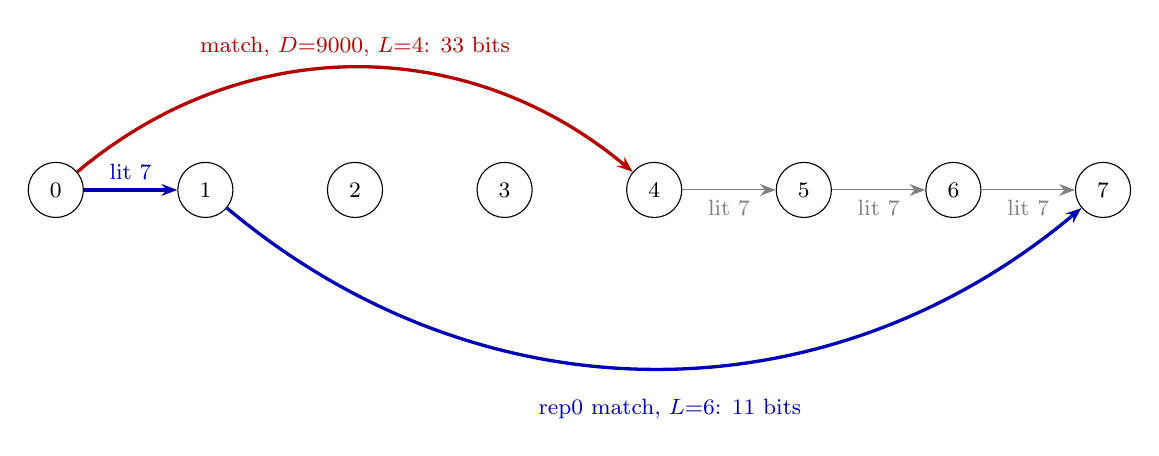
\begin{tikzpicture}[font=\footnotesize,
  n/.style={circle,draw,minimum size=0.7cm,fill=white,inner sep=0},
  >={Stealth[length=2mm]}]
\foreach \i in {0,...,7} {\node[n] (n\i) at (1.9*\i,0) {\i};}
\foreach \i/\j in {4/5,5/6,6/7} {\draw[->,gray] (n\i) -- node[below,gray] {lit 7} (n\j);}
\draw[->,very thick,red!70!black] (n0) to[bend left=40] node[above] {match, $D{=}9000$, $L{=}4$: 33 bits} (n4);
\draw[->,very thick,blue!70!black] (n1) to[bend right=40] node[below,xshift=0.2cm,yshift=-0.25cm] {rep0 match, $L{=}6$: 11 bits} (n7);
\draw[->,very thick,blue!70!black] (n0) -- node[above] {lit 7} (n1);
\end{tikzpicture}
\caption{A greedy parser takes the longest match at position~0 (red: 33 bits to reach position 4) and then must finish with literals:
$33+7+7+7=54$ bits. The optimal path (blue) takes one literal and then a repeated match: $7+11=18$ bits. The costs are illustrative, but costs of this magnitude (a fresh match with a far
distance is expensive, a rep match is cheap) are realistic.}
\label{fig:optimal}
\end{figure}

A practical optimal parser (the one in the LZMA SDK) works as follows:
\begin{enumerate}[leftmargin=2em]
\item At the current position, gather candidates: literal; all rep matches (rep0..rep3) with their lengths; all matches from the match finder (for each length, the nearest distance);
  and compound patterns such as ``literal followed by rep0 match'' or ``match, literal, rep0 match''.
\item Extend the search forward through the cheapest reachable positions, recording for each the best known cost and the packet and state that achieved it, until the window ends
  or a very long match (\code{nice_len}) is found.
\item Walk the best path back from the end and \emph{emit} those packets, updating the real probabilities and state, then continue from where the path ended.
\end{enumerate}
It is a heuristic, not a perfect shortest path: the price of an edge depends on the state and the rep history, which depend on the path taken, and the adaptive probabilities change as
packets are coded. Nevertheless it yields substantial gains over greedy parsing, as measured below.

\section{Presets}

\texttt{xz} presets $0$--$3$ use a faster mode with hash-chain match finders and simpler parsing; presets $4$--$9$ use binary trees and optimal parsing. Dictionary sizes and
approximate memory (from the \texttt{xz} manual; they may vary slightly between versions):
\begin{center}
\small
\begin{tabular}{rrrr}
\toprule
preset & dictionary & compressor memory & decompressor memory\\
\midrule
0 & 256 KiB & 3 MiB & 1 MiB\\
1 & 1 MiB & 9 MiB & 2 MiB\\
3 & 4 MiB & 32 MiB & 5 MiB\\
6 & 8 MiB & 94 MiB & 9 MiB\\
9 & 64 MiB & 674 MiB & 65 MiB\\
\bottomrule
\end{tabular}
\end{center}
Note the asymmetry: decompression needs memory roughly equal to the dictionary (the sliding window) plus about 16\,KiB of probabilities, while compression needs about
an order of magnitude more.

% =====================================================================
\chapter{Why LZMA Wins (and Where It Loses)}
% =====================================================================

\section{Measured comparison}

All numbers below were measured on one machine with Python's standard \texttt{zlib}, \texttt{bz2} and \texttt{lzma} modules, on two data sets. Timings are
indicative only; the point is the ratio of sizes.

\paragraph{Data set A (text).} 8\,000\,000 bytes: 574 Python source files concatenated.
\begin{center}
\small
\begin{tabular}{lrrr}
\toprule
compressor & size (bytes) & ratio & compression time\\
\midrule
zlib level 6 (Deflate) & 1\,770\,042 & 22.13\% & 0.26 s\\
zlib level 9 (Deflate) & 1\,746\,846 & 21.84\% & 1.02 s\\
bzip2 level 9 & 1\,373\,963 & 17.17\% & 0.62 s\\
LZMA preset 1 & 1\,538\,776 & 19.23\% & 0.49 s\\
LZMA preset 6 & \textbf{1\,253\,160} & \textbf{15.66\%} & 4.76 s\\
\bottomrule
\end{tabular}
\end{center}
Decompression of this set: Deflate 0.03\,s, LZMA 0.11\,s.

\paragraph{Data set B (binaries).} 6\,000\,000 bytes from executables in \texttt{/usr/bin}.
\begin{center}
\small
\begin{tabular}{lrrr}
\toprule
compressor & size (bytes) & ratio & compression time\\
\midrule
zlib level 9 & 2\,838\,509 & 47.31\% & 0.78 s\\
bzip2 level 9 & 2\,675\,845 & 44.60\% & 0.51 s\\
LZMA preset 6 & \textbf{2\,312\,984} & \textbf{38.55\%} & 3.49 s\\
\bottomrule
\end{tabular}
\end{center}

On the text LZMA produces output 28\% smaller than Deflate-9 and 9\% smaller than bzip2; on the binaries, 19\% and 14\% smaller respectively.

\section{Which ingredient matters how much?}

Using the real encoder with settings changed one at a time (data set A, LZMA2 raw streams, otherwise preset 6):

\begin{center}
\small
\begin{tabular}{lrr}
\toprule
configuration & size (bytes) & ratio\\
\midrule
default (dictionary 8 MiB, $\code{lc}=3,\code{lp}=0,\code{pb}=2$, optimal parsing) & 1\,253\,098 & 15.66\%\\
dictionary 32 KiB (the Deflate window) & 1\,575\,174 & 19.69\%\\
dictionary 256 KiB & 1\,365\,127 & 17.06\%\\
dictionary 1 MiB & 1\,302\,138 & 16.28\%\\
fast mode, \code{hc4}, \code{nice_len}=64 (no optimal parsing) & 1\,476\,349 & 18.45\%\\
normal mode, \code{nice_len}=8 (short search) & 1\,537\,379 & 19.22\%\\
normal mode, \code{nice_len}=273 & 1\,249\,222 & 15.62\%\\
$\code{lc}=0$ & 1\,257\,114 & 15.71\%\\
$\code{lc}=4$ & 1\,252\,291 & 15.65\%\\
$\code{pb}=0$ & 1\,250\,636 & 15.63\%\\
\bottomrule
\end{tabular}
\end{center}

Observations (all specific to this data set, and worth repeating on your own data):
\begin{itemize}
\item \textbf{The dictionary matters a lot} on this data: shrinking it to Deflate's 32\,KiB costs 26\% more output.
\item \textbf{Search and parsing effort matter a lot}: the fast mode is 18\% larger than the optimal-parsing mode, and a shallow search is 23\% larger.
\item \textbf{\code{lc}, \code{lp}, \code{pb} matter little for source text} (differences of a few tenths of a percent) but can matter much more for structured binary data. Context bits
are not magic; each costs learning time.
\end{itemize}
The remaining advantage over Deflate comes from the range coder and the context modelling (flags conditioned on state and position, matched literals, rep matches), which does not show up in an
ablation of tuning parameters but is built into the format. It is why even a 32\,KiB-dictionary LZMA stream is smaller than a Deflate stream with a similar window (1\,575\,174 bytes against 1\,746\,846 here).

\section{The summary}

\begin{center}
\small
\begin{tabular}{p{3.6cm}p{5.2cm}p{5.2cm}}
\toprule
 & Deflate (gzip) & LZMA\\
\midrule
Window & 32 KiB & MiB to GiB\\
Entropy coder & Huffman trees per block, sent in the stream & adaptive binary range coder, no side information\\
Cost floor per decision & 1 bit & about 0.02 bits\\
Literal modelling & none (a single tree) & context: previous byte, position bits, expected byte after a match\\
Distance modelling & fixed code classes, extra bits raw & slot tree by length class, align bits, 4 repeat distances\\
Parsing & greedy / lazy & optimal (price-based dynamic programming)\\
Decoder speed & very fast & moderate (serial bit-by-bit)\\
Compression speed & fast & slow\\
\bottomrule
\end{tabular}
\end{center}

\section{Limitations}

\begin{itemize}
\item \textbf{Decoding is inherently serial.} Each decision depends on the adaptive state left by all previous ones. You cannot start decoding in the middle of a chunk, which
is why LZMA2 and \texttt{xz} introduce independent blocks for multi-threading.
\item \textbf{Slower than modern LZ codecs.} Zstandard and LZ4 decode several times faster, with Zstandard at its higher levels coming close to LZMA ratios on many data sets.
LZMA's niche is ``compress once, ship many times, minimise size''.
\item \textbf{Compressor memory} can be hundreds of MiB at high presets.
\item \textbf{Incompressible data} is expanded slightly by plain LZMA (LZMA2 avoids this with stored chunks).
\item \textbf{Not suitable for very small inputs}, since the models start untrained (Chapter~9).
\end{itemize}

% =====================================================================
\chapter{Exercises}
% =====================================================================

Solutions follow. Try them first; use the decoder in Appendix~A for experiments.

\begin{enumerate}[label=\textbf{E\arabic*.},leftmargin=2.4em,itemsep=0.7em]
\item \textbf{Range coder step.} The encoder has $\code{range}=\hex{10000000}$, $\code{prob}=1500$, and codes a \bits{1}. Compute \code{bound}, the new \code{range}, the new \code{prob}, and the
  increase of \code{low}. Is normalisation needed?
\item \textbf{Distance coding.} Code the distance $D=300$: give $d$, the slot, the number of extra bits, the base, the extra value, and how the extra bits are coded.
\item \textbf{State machine.} Starting at state 0, the packets are LIT, MATCH, LIT, LIT, LONGREP, SHORTREP. Give the state after each packet.
\item \textbf{Properties byte.} (a) Decode the properties byte \hex{5D}. (b) Compute the byte for $\code{lc}=0,\ \code{lp}=2,\ \code{pb}=2$.
\item \textbf{Memory of the model.} How many probabilities does a decoder with $\code{lc}=3$, $\code{lp}=0$ need? How many bytes if each is 16 bits?
\item \textbf{Length coding.} Describe the decisions coded for $L=2$, $L=9$, $L=10$, $L=18$ and $L=273$.
\item \textbf{Cost of a decision.} A flag has probability 1990/2048 of being \bits{0}. What does coding a \bits{0} cost, and a \bits{1}?
\item \textbf{Parsing.} The text \texttt{xyzxyzxyzxyz} (12 bytes) is given. Find a short packet sequence. How does the overlapping-copy rule help?
\item \textbf{Thinking question.} Why does the range coder use only the \emph{high} bits of \code{range} to compute \code{bound}, and why must the probability never reach 0 or 2048?
\item \textbf{Challenge.} Modify the C decoder in Appendix~A to count how many packets of each type (LIT, MATCH, SHORTREP, LONGREP[0--3]) a stream contains. Run it on files produced by \code{xz --format=lzma} for some text file and for an executable. What is
  the typical ratio of literals to matches? How common are rep matches?
\end{enumerate}

\chapter*{Solutions}
\addcontentsline{toc}{chapter}{Solutions to the exercises}

\begin{enumerate}[label=\textbf{S\arabic*.},leftmargin=2.4em,itemsep=0.7em]
\item $\code{range}\gg11=2^{28}/2^{11}=131\,072$; $\code{bound}=131\,072\times1500=196\,608\,000$. Bit \bits{1}: $\code{low}$ increases by $196\,608\,000$; $\code{range}=268\,435\,456-196\,608\,000=71\,827\,456$;
  $\code{prob}=1500-(1500\gg5)=1500-46=1454$. Since $71\,827\,456>2^{24}=16\,777\,216$, no normalisation.
\item $d=299=\bits{100101011}$ (9 bits), $n=8$, next bit $0$, slot $=16$. $n_x=(16\gg1)-1=7$, base $=2\ll7=256$, extra $=299-256=43=\bits{0101011}$. Slot $\ge14$: top $7-4=3$ bits \bits{010} as direct bits, low 4 bits \bits{1011}
  with the \code{align} reverse tree (coded LSB first: 1,1,0,1).
\item LIT: 0; MATCH: 7; LIT: $7\to4$; LIT: $4\to1$; LONGREP: $1<7\to8$; SHORTREP: $8\ge7\to11$. Sequence: 0, 7, 4, 1, 8, 11.
\item (a) $93=(\code{pb}\cdot5+\code{lp})\cdot9+\code{lc}$: $93=10\cdot9+3$, so $\code{lc}=3$, and $10=\code{pb}\cdot5+\code{lp}$ gives $\code{pb}=2,\code{lp}=0$. (b) $(2\cdot5+2)\cdot9+0=108=\hex{6C}$.
\item $1846+768\cdot2^{\code{lc}+\code{lp}}=1846+768\cdot8=7990$ probabilities; $\times2$ bytes $=15\,980$ bytes, about 15.6\,KiB. (The 1846 base: $192+48+192+256+114+16+1028$ for the \code{isMatch}, rep flags, \code{isRep0Long}, slot trees, special positions, align, and two length coders; see Appendix~B.)
\item $L=2$: \code{choice}=0, \code{low} value 0 (\bits{000}). $L=9$: \code{choice}=0, \code{low} value 7 (\bits{111}). $L=10$: \code{choice}=1, \code{choice2}=0, \code{mid} value 0. $L=18$: \code{choice}=1, \code{choice2}=1, \code{high} value 0 (8 zeros).
  $L=273$: \code{choice}=1, \code{choice2}=1, \code{high} value 255.
\item $P(0)=1990/2048=0.9717$: coding \bits{0} costs $-\log_2 0.9717=0.041$ bits; coding \bits{1} has probability $58/2048=0.0283$ and costs $-\log_2 0.0283=5.14$ bits. A confident model is cheap when right, and expensive (but not catastrophic) when wrong.
\item Literals \texttt{x y z}, then one match with $D=3$ and $L=9$: $3+1$ packets for 12 bytes. Because the copy goes byte by byte, the match source overlaps the destination ($L>D$), and the 3-byte pattern repeats itself.
\item The product $(\code{range}\gg11)\times\code{prob}$ fits in 32 bits because $\code{prob}<2^{11}$. If \code{prob} could reach 0 or 2048, \code{bound} would be 0 or \code{range}, making one outcome impossible (a zero-width interval) and the stream undecodable if that outcome occurred. The update rule's integer rounding keeps $\code{prob}\in[31,2017]$.
\item (Open-ended.) For ordinary text expect matches to be a minority of packets but to cover most of the bytes; rep matches are typically a significant fraction of matches in source code and structured data.
\end{enumerate}

\appendix
% =====================================================================
\chapter{A Complete LZMA Decoder in C}
% =====================================================================

The following decoder handles the \texttt{.lzma} (``LZMA-alone'') format and is about 200 lines of plain C99 with no dependencies. I tested it against files produced by the real
\texttt{xz} tool (which uses liblzma) for presets \texttt{-0}, \texttt{-3}, \texttt{-6} and \texttt{-9e} on seven inputs (the 15-byte sample string, an empty file, 20\,000 random bytes,
a 100\,000-byte run, repeated source text, 600\,KB of executable code, and a 4.6\,MB collection of source files), and with non-default settings (\code{lc}/\code{lp}/\code{pb} = 0/2/2, 4/0/0 and 1/3/4). Every output matched the original byte for byte, and
all runs were clean under AddressSanitizer and UBSan. It favours clarity over speed (the whole output is kept in memory and serves as the dictionary), and every part corresponds to a section above.

\begin{center}
\small
\begin{tabular}{ll}
\toprule
code & explained in\\
\midrule
\code{rc_bit}, \code{normalize} & Chapter 4 (decoding one bit, adaptation, normalisation)\\
\code{rc_direct}, \code{rc_tree}, \code{rc_rtree} & Chapter 4 (direct bits, bit trees, reverse trees)\\
\code{LenDec}, \code{len_decode} & Chapter 7 (length coder)\\
main loop, \code{state} updates & Chapter 5 (packets, state machine)\\
matched literal branch & Chapter 6\\
\code{slot}, \code{dist} computation & Chapter 7 (distance coder)\\
\code{rep[]} handling & Chapter 8\\
\bottomrule
\end{tabular}
\end{center}

\begin{lstlisting}[language=C,caption={\texttt{lzma\_dec.c}: reference LZMA decoder (tested).}]
/* lzma_dec.c - minimal reference decoder for the .lzma ("LZMA-alone") format.
 * Clarity over speed. Build:  gcc -O2 -Wall -o lzma_dec lzma_dec.c
 * Usage: ./lzma_dec input.lzma output.bin                                    */
#include <stdint.h>
#include <stdio.h>
#include <stdlib.h>
#include <string.h>

typedef uint16_t Prob;
#define TOP_VALUE (1u << 24)

static void die(const char *msg) { fprintf(stderr, "error: %s\n", msg); exit(1); }

static void init_probs(Prob *p, size_t n) { while (n--) *p++ = 1024; }

/* ---------------- range decoder (Chapter 4) ---------------- */
typedef struct { const uint8_t *in, *end; uint32_t range, code; } RC;

static uint8_t next_byte(RC *rc) {
    if (rc->in >= rc->end) die("truncated input");
    return *rc->in++;
}
static void rc_init(RC *rc, const uint8_t *in, const uint8_t *end) {
    rc->in = in; rc->end = end; rc->range = 0xFFFFFFFFu; rc->code = 0;
    if (next_byte(rc) != 0) die("first range-coder byte must be 0");
    for (int i = 0; i < 4; i++) rc->code = (rc->code << 8) | next_byte(rc);
}
static void normalize(RC *rc) {
    if (rc->range < TOP_VALUE) {
        rc->range <<= 8;
        rc->code = (rc->code << 8) | next_byte(rc);
    }
}
/* decode one bit with adaptive probability *p */
static int rc_bit(RC *rc, Prob *p) {
    uint32_t bound = (rc->range >> 11) * *p;
    int bit;
    if (rc->code < bound) { rc->range = bound;  *p += (2048 - *p) >> 5; bit = 0; }
    else { rc->range -= bound; rc->code -= bound; *p -= *p >> 5;        bit = 1; }
    normalize(rc);
    return bit;
}
/* n bits with fixed probability 1/2 */
static uint32_t rc_direct(RC *rc, int n) {
    uint32_t r = 0;
    while (n--) {
        rc->range >>= 1;
        uint32_t b = rc->code >= rc->range;
        if (b) rc->code -= rc->range;
        r = (r << 1) | b;
        normalize(rc);
    }
    return r;
}
/* bit tree, MSB first; probs has 2^nbits entries (index 0 unused) */
static uint32_t rc_tree(RC *rc, Prob *probs, int nbits) {
    uint32_t m = 1;
    for (int i = 0; i < nbits; i++) m = (m << 1) | rc_bit(rc, &probs[m]);
    return m - (1u << nbits);
}
/* reverse bit tree, LSB first */
static uint32_t rc_rtree(RC *rc, Prob *probs, int nbits) {
    uint32_t m = 1, sym = 0;
    for (int i = 0; i < nbits; i++) {
        uint32_t b = rc_bit(rc, &probs[m]);
        m = (m << 1) | b;
        sym |= b << i;
    }
    return sym;
}

/* ---------------- length coder (Chapter 7) ---------------- */
typedef struct { Prob choice, choice2, low[16][8], mid[16][8], high[256]; } LenDec;

static void len_init(LenDec *l) { init_probs((Prob *)l, sizeof *l / sizeof(Prob)); }
static uint32_t len_decode(RC *rc, LenDec *l, unsigned pos_state) {
    if (!rc_bit(rc, &l->choice))  return 2  + rc_tree(rc, l->low[pos_state], 3);
    if (!rc_bit(rc, &l->choice2)) return 10 + rc_tree(rc, l->mid[pos_state], 3);
    return 18 + rc_tree(rc, l->high, 8);
}

/* ---------------- output buffer (the whole output is the dictionary) ---------------- */
typedef struct { uint8_t *buf; size_t len, cap; } Out;
static void out_put(Out *o, uint8_t b) {
    if (o->len == o->cap) {
        o->cap = o->cap ? o->cap * 2 : 4096;
        o->buf = realloc(o->buf, o->cap);
        if (!o->buf) die("out of memory");
    }
    o->buf[o->len++] = b;
}

/* ---------------- main decoder ---------------- */
static Out lzma_alone_decode(const uint8_t *data, size_t size) {
    if (size < 13) die("file too short");
    unsigned d = data[0];
    if (d >= 9 * 5 * 5) die("bad properties byte");
    unsigned lc = d % 9; d /= 9;
    unsigned lp = d % 5; unsigned pb = d / 5;
    uint64_t usize = 0;
    for (int i = 0; i < 8; i++) usize |= (uint64_t)data[5 + i] << (8 * i);
    int unknown = (usize == UINT64_MAX);

    RC rc; rc_init(&rc, data + 13, data + size);

    size_t nlit = (size_t)0x300 << (lc + lp);
    Prob *literal = malloc(nlit * sizeof(Prob));
    if (!literal) die("out of memory");
    init_probs(literal, nlit);

    Prob is_match[12][16], is_rep[12], is_rep_g0[12], is_rep_g1[12], is_rep_g2[12];
    Prob is_rep0_long[12][16], pos_slot[4][64], pos_special[115], align[16];
    init_probs(&is_match[0][0], 12 * 16);  init_probs(is_rep, 12);
    init_probs(is_rep_g0, 12); init_probs(is_rep_g1, 12); init_probs(is_rep_g2, 12);
    init_probs(&is_rep0_long[0][0], 12 * 16);
    init_probs(&pos_slot[0][0], 4 * 64);   init_probs(pos_special, 115);
    init_probs(align, 16);
    LenDec len_dec, rep_len_dec; len_init(&len_dec); len_init(&rep_len_dec);

    Out out = {0};
    unsigned state = 0;
    uint32_t rep[4] = {0, 0, 0, 0};

    while (unknown || out.len < usize) {
        size_t pos = out.len;
        unsigned ps = pos & ((1u << pb) - 1);

        if (!rc_bit(&rc, &is_match[state][ps])) {                 /* ---- literal */
            unsigned prev = pos ? out.buf[pos - 1] : 0;
            Prob *probs = literal + 0x300 * (((pos & ((1u << lp) - 1)) << lc) + (prev >> (8 - lc)));
            unsigned sym = 1;
            if (state >= 7) {                                      /* matched literal */
                unsigned mb = out.buf[pos - rep[0] - 1];
                while (sym < 0x100) {
                    unsigned match_bit = (mb >> 7) & 1; mb <<= 1;
                    unsigned bit = rc_bit(&rc, &probs[((1 + match_bit) << 8) + sym]);
                    sym = (sym << 1) | bit;
                    if (match_bit != bit) break;
                }
            }
            while (sym < 0x100) sym = (sym << 1) | rc_bit(&rc, &probs[sym]);
            out_put(&out, (uint8_t)sym);
            state = state < 4 ? 0 : (state < 10 ? state - 3 : state - 6);
            continue;
        }

        uint32_t len;
        if (!rc_bit(&rc, &is_rep[state])) {                        /* ---- simple match */
            rep[3] = rep[2]; rep[2] = rep[1]; rep[1] = rep[0];
            len = len_decode(&rc, &len_dec, ps);
            state = state < 7 ? 7 : 10;
            uint32_t slot = rc_tree(&rc, pos_slot[len - 2 < 3 ? len - 2 : 3], 6);
            uint32_t dist;
            if (slot < 4) dist = slot;
            else {
                int nd = (slot >> 1) - 1;
                dist = (2 | (slot & 1)) << nd;
                if (slot < 14) dist += rc_rtree(&rc, pos_special + dist - slot, nd);
                else {
                    dist += rc_direct(&rc, nd - 4) << 4;
                    dist += rc_rtree(&rc, align, 4);
                }
            }
            if (dist == 0xFFFFFFFFu) break;                        /* end marker */
            rep[0] = dist;
        } else {                                                   /* ---- rep match */
            if (!rc_bit(&rc, &is_rep_g0[state])) {
                if (!rc_bit(&rc, &is_rep0_long[state][ps])) {      /* short rep */
                    state = state < 7 ? 9 : 11;
                    if (rep[0] >= pos) die("bad distance");
                    out_put(&out, out.buf[pos - rep[0] - 1]);
                    continue;
                }
            } else {
                uint32_t dist;
                if (!rc_bit(&rc, &is_rep_g1[state])) dist = rep[1];
                else {
                    if (!rc_bit(&rc, &is_rep_g2[state])) dist = rep[2];
                    else { dist = rep[3]; rep[3] = rep[2]; }
                    rep[2] = rep[1];
                }
                rep[1] = rep[0]; rep[0] = dist;
            }
            len = len_decode(&rc, &rep_len_dec, ps);
            state = state < 7 ? 8 : 11;
        }
        if (rep[0] >= pos) die("bad distance");
        if (!unknown && len > usize - out.len) die("match exceeds declared size");
        for (uint32_t i = 0; i < len; i++)                         /* byte-by-byte copy */
            out_put(&out, out.buf[out.len - rep[0] - 1]);
    }
    free(literal);
    return out;
}

int main(int argc, char **argv) {
    if (argc != 3) { fprintf(stderr, "usage: %s in.lzma out\n", argv[0]); return 2; }
    FILE *f = fopen(argv[1], "rb");
    if (!f) die("cannot open input");
    fseek(f, 0, SEEK_END); long n = ftell(f); fseek(f, 0, SEEK_SET);
    uint8_t *data = malloc(n > 0 ? n : 1);
    if (!data || fread(data, 1, n, f) != (size_t)n) die("read failed");
    fclose(f);
    Out out = lzma_alone_decode(data, (size_t)n);
    FILE *g = fopen(argv[2], "wb");
    if (!g) die("cannot open output");
    if (out.len && fwrite(out.buf, 1, out.len, g) != out.len) die("write failed");
    fclose(g);
    free(out.buf); free(data);
    return 0;
}
\end{lstlisting}

\paragraph{Building and testing.}
\begin{lstlisting}[language=bash]
gcc -O2 -Wall -o lzma_dec lzma_dec.c
echo -n "abcdXabcdYabcdZ" > sample.txt
xz --format=lzma -c sample.txt > sample.lzma     # 33 bytes, as in Chapter 9
./lzma_dec sample.lzma roundtrip.txt
cmp sample.txt roundtrip.txt && echo identical
\end{lstlisting}

\chapter{Cheat Sheet of Constants and Contexts}

\section{Probability arrays}

All probabilities are 11-bit, initialised to 1024; adaptation shift is 5.

\begin{center}
\small
\begin{tabular}{p{4.8cm}p{6.2cm}r}
\toprule
array & indexed by & number of probabilities\\
\midrule
\code{isMatch} & state (12), posState (16) & 192\\
\code{isRep}, \code{isRepG0}, \code{isRepG1}, \code{isRepG2} & state (12) & $4\times12=48$\\
\code{isRep0Long} & state (12), posState (16) & 192\\
\code{posSlot} & lenState (4), 6-bit tree (64) & 256\\
\code{posSpecial} & reverse trees for slots 4--13 & 114\\
\code{align} & 4-bit reverse tree & 16\\
length coder (two of them) & choice 2, low $16\times8$, mid $16\times8$, high 256 & $2\times514=1028$\\
\midrule
\multicolumn{2}{l}{subtotal (independent of \code{lc}, \code{lp})} & 1846\\
\code{literal} & $2^{\code{lc}+\code{lp}}$ contexts $\times\ \hex{300}$ & $768\cdot2^{\code{lc}+\code{lp}}$\\
\bottomrule
\end{tabular}
\end{center}

(The number of posState values actually used is $2^{\code{pb}}$; the arrays are sized for the maximum, $\code{pb}=4$.)

\section{Numeric constants}

\begin{center}
\small
\begin{tabular}{p{4.6cm}p{10.4cm}}
\toprule
probability bits & 11 (probabilities in $[0,2048)$, start 1024)\\
adaptation shift & 5\\
probability limits in practice & 31 to 2017\\
range-coder top value & $2^{24}$ (normalise when \code{range} falls below it)\\
initial range & \hex{FFFFFFFF}\\
minimum / maximum match length & 2 / 273\\
state count & 12 (literal states 0--6, match states 7--11)\\
distance slots & 64 (slots $<4$: no extra bits; $4$--$13$: modelled; $\ge14$: direct + 4 align)\\
end-of-payload marker & distance \hex{FFFFFFFF} (slot 63, all extra bits 1)\\
default properties & $\code{lc}=3,\ \code{lp}=0,\ \code{pb}=2$ = byte \hex{5D}\\
\bottomrule
\end{tabular}
\end{center}

\chapter{Further Reading}

\begin{itemize}
\item Igor Pavlov, \emph{LZMA SDK} and the accompanying \texttt{lzma-specification} document (public domain); the C and C++ sources are the ultimate reference.
\item Lasse Collin, \emph{The .xz File Format} specification, and the \texttt{xz}/liblzma sources (the encoder, match finders and presets).
\item J.\ Ziv and A.\ Lempel, ``A Universal Algorithm for Sequential Data Compression'', \emph{IEEE Transactions on Information Theory}, 1977 (LZ77).
\item C.\ E.\ Shannon, ``A Mathematical Theory of Communication'', 1948.
\item G.\ N.\ N.\ Martin, ``Range encoding: an algorithm for removing redundancy from a digitised message'', 1979; and J.\ Rissanen and G.\ Langdon, ``Arithmetic coding'', \emph{IBM Journal of Research and Development}, 1979.
\item Matt Mahoney, \emph{Data Compression Explained}, an online book covering context modelling and arithmetic coding.
\end{itemize}

\end{document}
